% 学習結果説明（手順3c：最終候補を MCMC で推定。用語集と図の見方）
% results フォルダで「lualatex 学習結果説明_手順3c.tex」を2回実行すると PDF を作り直せる（TeX Live の LuaLaTeX を使用）。
% 図は results/step3c_mcmc/ の PNG を相対パスで読み込む。
\documentclass[paper=a4paper,fontsize=10.5pt,line_length=44zw,number_of_lines=38]{jlreq}
\usepackage[haranoaji]{luatexja-preset}
\usepackage{amsmath}
\usepackage{graphicx}
\usepackage{booktabs}
\usepackage{tabularx}
\usepackage{enumitem}
\usepackage{float}
\usepackage{xcolor}
\usepackage[hidelinks,bookmarksnumbered]{hyperref}
\graphicspath{{step3c_mcmc/}}

\newcommand{\file}[1]{\texttt{\detokenize{#1}}}
\newcommand{\gd}{\dot{\gamma}}
\newcommand{\Tff}{T_{\mathrm{ff}}}
\newcommand{\Tset}{T_{\mathrm{set}}}
\newenvironment{termlist}{\begin{itemize}[label=・,leftmargin=1\zw,labelwidth=1\zw,labelsep=0pt,itemsep=0.4ex,topsep=0.6ex,parsep=0pt]}{\end{itemize}}
\newcommand{\term}[1]{\item \textbf{#1}：}
\newenvironment{points}{\begin{itemize}[label=$\triangleright$,leftmargin=1.5\zw,itemsep=0.3ex,topsep=0.5ex,parsep=0pt]}{\end{itemize}}
\newcommand{\pt}[1]{\item \textbf{#1}：}
\renewcommand{\arraystretch}{1.25}

\title{樹脂粘度モデル開発　手順3cの学習結果の説明\\[0.6ex]{\large 最終候補のモデルを MCMC で推定：用語集とグラフの見方（機械学習・統計を初めて学ぶ人向け）}}
\author{}
\date{2026年10月13日}

\begin{document}
\maketitle
{\small\tableofcontents}

% =====================================================================
\section{この文書について}

この文書は、\file{results/step3c_mcmc/} にある手順3cの結果（図と表）を、機械学習や統計を初めて学ぶ人でも読めるように説明したものです。手順2の MCMC 版の説明は、\file{学習結果説明.pdf} の用語集にあります。この文書は、それと重なる用語を短く繰り返し、新しい用語を足しています。

\begin{points}
\pt{対象の結果}\file{results/step3c_mcmc/}：手順3bで決めた最終候補のモデル（B0T、R3、R2）の、ハイパーパラメータを、MCMC で推定した結果です（図 20 枚、CSV 6 個、事後サンプル 12 個）。最尤推定と比べて、何が変わるかを調べました。
\pt{読み方}2章で何をしたかをつかみ、分からない言葉は3章の用語集で調べてください。4章で図の見方、5章で表の見方、6章で結果のまとめを説明します。
\pt{数値について}文中の数値は、この文書を作った時点の results の表から取り出したものです。
\pt{元のノート}\file{01_機械学習コードフォルダ} の \file{手順3c_最終候補のMCMC.ipynb} です。ノートの先頭に使い方があり、「設定エリア」だけを直せば設定を変えられます。サンプリングには、全体で約 46 分かかります（保存済みのサンプルがあれば、それを読み込んで省けます）。報告書・発表資料用の高解像度のグラフ（せん断速度 ― 粘度）は、ノート9章のセルで作ります（4章の最後）。
\pt{記号表}記号・モデル名（B0T、R3、R2 など）・列名の一覧は、\file{学習結果説明_記号表.pdf} にあります。
\pt{作り直し方}\file{results} フォルダで \texttt{lualatex 学習結果説明\_手順3c.tex} を2回実行すると、この PDF を作り直せます。
\end{points}

% =====================================================================
\section{何をしたか（概要）}

\subsection{目的}
手順3bまでは、ハイパーパラメータ（振幅・長さスケール・ノイズ分散など）を、データが最も「ありそう」になる1組の値（\textbf{最尤推定}）に決めていました。1組だけを使うと、次の2つの心配があります。

\begin{points}
\pt{心配1：最適化が、悪い所で止まる}最適化は、近くの「谷」で止まることがあります。手順3bで、PP の S\_T の B0T がそうでした（$\Tset$ の長さスケールが下限に張り付き、210 ℃ を内挿できませんでした）。
\pt{心配2：ハイパーパラメータの不確かさを無視している}データが少ないと、ハイパーパラメータは1つの値に決まりきりません。1組だけで予測すると、予測の幅が狭すぎるかもしれません。
\end{points}

\textbf{MCMC}（マルコフ連鎖モンテカルロ法）は、ハイパーパラメータを1組に決めず、「ありそうな値の分布（事後分布）」を求める方法です。予測は、その分布からたくさん取り出した値で予測した結果を、混ぜて出します。これで2つの心配を調べます。手順5の本実装に使う形のモデルだけを、ここで MCMC にかけます（CLAUDE.md §5：最終候補だけ MCMC）。

\subsection{候補のモデルと、分け方}
\begin{table}[H]
\caption{最終候補のモデル（ARD Matern 5/2 ＋ 線形カーネル ＋ ノイズ。入力は $\ln$ をとった値で、$\Tset$ は ℃）}
\begin{tabularx}{\linewidth}{@{}l>{\raggedright\arraybackslash}p{15\zw}X@{}}
\toprule
記号 & 入力 & 選んだ理由 \\
\midrule
B0T & ショットごとの $\gd$，$H$，$\Tset$ & 手順3bで、PP の S\_T で最適化が失敗したモデル。MCMC で直るかを見る。 \\
R3 & 条件平均の $\gd$，$H$，$\Tset$ & 手順3bの結論で、基本とするモデル。 \\
R2 & 射出速度 $v$，$H$，$\Tset$ & 設定値だけで予測できるか（実測の $\gd$ を使わない）。 \\
\bottomrule
\end{tabularx}
\end{table}

$\Tff$ や \texttt{P3\_2} を足したモデルは、手順3bで要らないと分かったので、入れていません。分け方は、S\_V（5data で学習して 3data で検証）と、S\_T（190・230 ℃ で学習して 210 ℃ を予測。3data の 210 ℃ は S\_T3）です。材料は PP と粉砕材混合 PP の2つなので、モデル 3 × 分け方 2 × 材料 2 ＝ 12 組です。

\subsection{MCMC の方法（手順2と同じ、自作の適応型メトロポリス法）}
\begin{enumerate}[itemsep=0.4ex,topsep=0.5ex]
\item 今いる値（ハイパーパラメータの組）の近くに、ランダムに候補を出す。
\item 候補のほうが「ありそう」（対数周辺尤度が大きい）なら、そこへ移る。そうでなくても、確率的に移ることがある。移らなければ、その場にとどまる。
\item これを何千回も繰り返すと、「ありそうな値」を、ありそうな度合いに比例した頻度で訪れる。その足跡が、事後分布。
\item 最初の 3,000 回（\textbf{調整期間}）は、足跡から、候補の出し方（ばらつきの大きさ・向き）を学び、採択率が 0.234 に近づくよう合わせる。この期間の足跡は捨てる。
\item 本番は 8,000 回。チェーン（別々の出発点から歩く足跡）は 4 本。収束していなければ（R-hat が 1.01 を超える、または有効サンプル数が 400 に届かない）、本番を 20,000 回に増やして、やり直す。
\end{enumerate}

\textbf{事前分布}は、カーネルの探索範囲（振幅 $10^{-3}$〜$10^{3}$、長さスケール $10^{-2}$〜$10^{2}$、線形項の振幅と $\sigma_0$、ノイズ分散 $10^{-6}$〜$10$）の中で、対数をとって一様です。範囲の中では、事後分布は尤度に比例するので、最も高い所は、最尤推定と一致します。

\textbf{予測}は、事後サンプルを等間隔に 200 個選び、それぞれのハイパーパラメータで GPR を作って予測し（ノイズ込みの正規分布）、200 個の分布を等しい重みで混ぜた「混合分布」で行います。

% =====================================================================
\section{用語集}

\subsection{MCMC に関する用語}
\begin{termlist}
\term{事後分布}データを見たあとの、「ハイパーパラメータが、どの値でありそうか」の分布。山の中心がありそうな値、山の幅が不確かさです。最尤推定は、この山の頂上の 1 点にあたります。
\term{事前分布}データを見る前の、「どの値でありそうか」の分布。ここでは、探索範囲の中で、対数をとって一様（どの桁も同じ重み）にしました。
\term{マルコフ連鎖・チェーン}今の値だけから、次の値が決まる、値の列。MCMC では、この列（足跡）を「チェーン」と呼び、別々の出発点から 4 本歩かせます。
\term{調整期間（ウォームアップ）}出発点の影響を消し、候補の出し方を学ぶ最初の期間。サンプルとしては使いません（3,000 回）。
\term{採択率}候補に移れた割合。小さすぎると足跡が動かず、大きすぎると小さな歩幅しか出ていません。0.234 前後が、目安です。
\term{R-hat（アールハット）}4 本のチェーンの足跡が、同じ分布に収まっているかの目安。1.00 に近いほど、一致しています。1.01 以下が目標です。
\term{有効サンプル数（ESS）}足跡は、前後で似ているので、「独立なサンプル何個分の情報があるか」を表す数。400 以上が目標です。値が小さいと、分布が粗くしか分かりません。
\term{トレース図}チェーンの値を、反復の順に描いた図。同じ範囲を上下して、4 本が混ざっていれば、収束しています。
\term{多峰性（複数の山）}事後分布に、離れた山が複数あること。チェーンは、山の間を行き来しにくく、R-hat が大きくなります。
\term{混合分布}たくさんの正規分布を、等しい重みで混ぜた分布。ここでは、事後サンプルごとの予測分布を混ぜたもの。ハイパーパラメータの不確かさを、予測の幅に入れられます。
\term{最尤推定と MCMC}最尤推定は、尤度が最大の 1 点。MCMC は、尤度に比例した分布全体。山が 1 つで尖っていれば、同じ結果になります。
\end{termlist}

\subsection{評価と、ハイパーパラメータに関する用語}
\begin{termlist}
\term{RMSE・被覆率・NLPD}手順3a・3bの用語集と同じです。RMSE は予測の平均的な誤差（$\ln\eta$）、被覆率は 95\% 予測区間に実測が入った割合、NLPD は予測の当たり具合と区間の適切さをまとめた指標（小さいほど良い）です。MCMC では、混合分布の平均・累積分布・密度で計算します。
\term{長さスケール}入力がどれだけ変わると出力が大きく変わるかの目安（標準化した入力に対する値）。探索範囲は $10^{-2}$〜$10^{2}$。上限に近いと、その入力はほとんど使われていません。
\term{線形カーネルの $\sigma_0$ と振幅}線形カーネル（$\sigma_0^2 + x\cdot x'$ に振幅の 2 乗を掛けたもの）のパラメータ。目的変数を中心化し、入力を標準化しているので、定数の項（$\sigma_0$）は、データでほとんど決まらず、事後分布が探索範囲いっぱいに広がります（予測にはほとんど効きません）。
\term{感度確認}手順3bの用語集と同じです。
\end{termlist}

% =====================================================================
\section{図の見方}

図ごとに、「何を示す図か」「軸と記号」「見るポイント」「今回の結果」の順に説明します。図のファイルは \file{results/step3c_mcmc/} にあります。

% ---------------------------------------------------------------------
\subsection{トレース図（\file{fig\_trace\_*.png}）}
\begin{figure}[H]
\centering
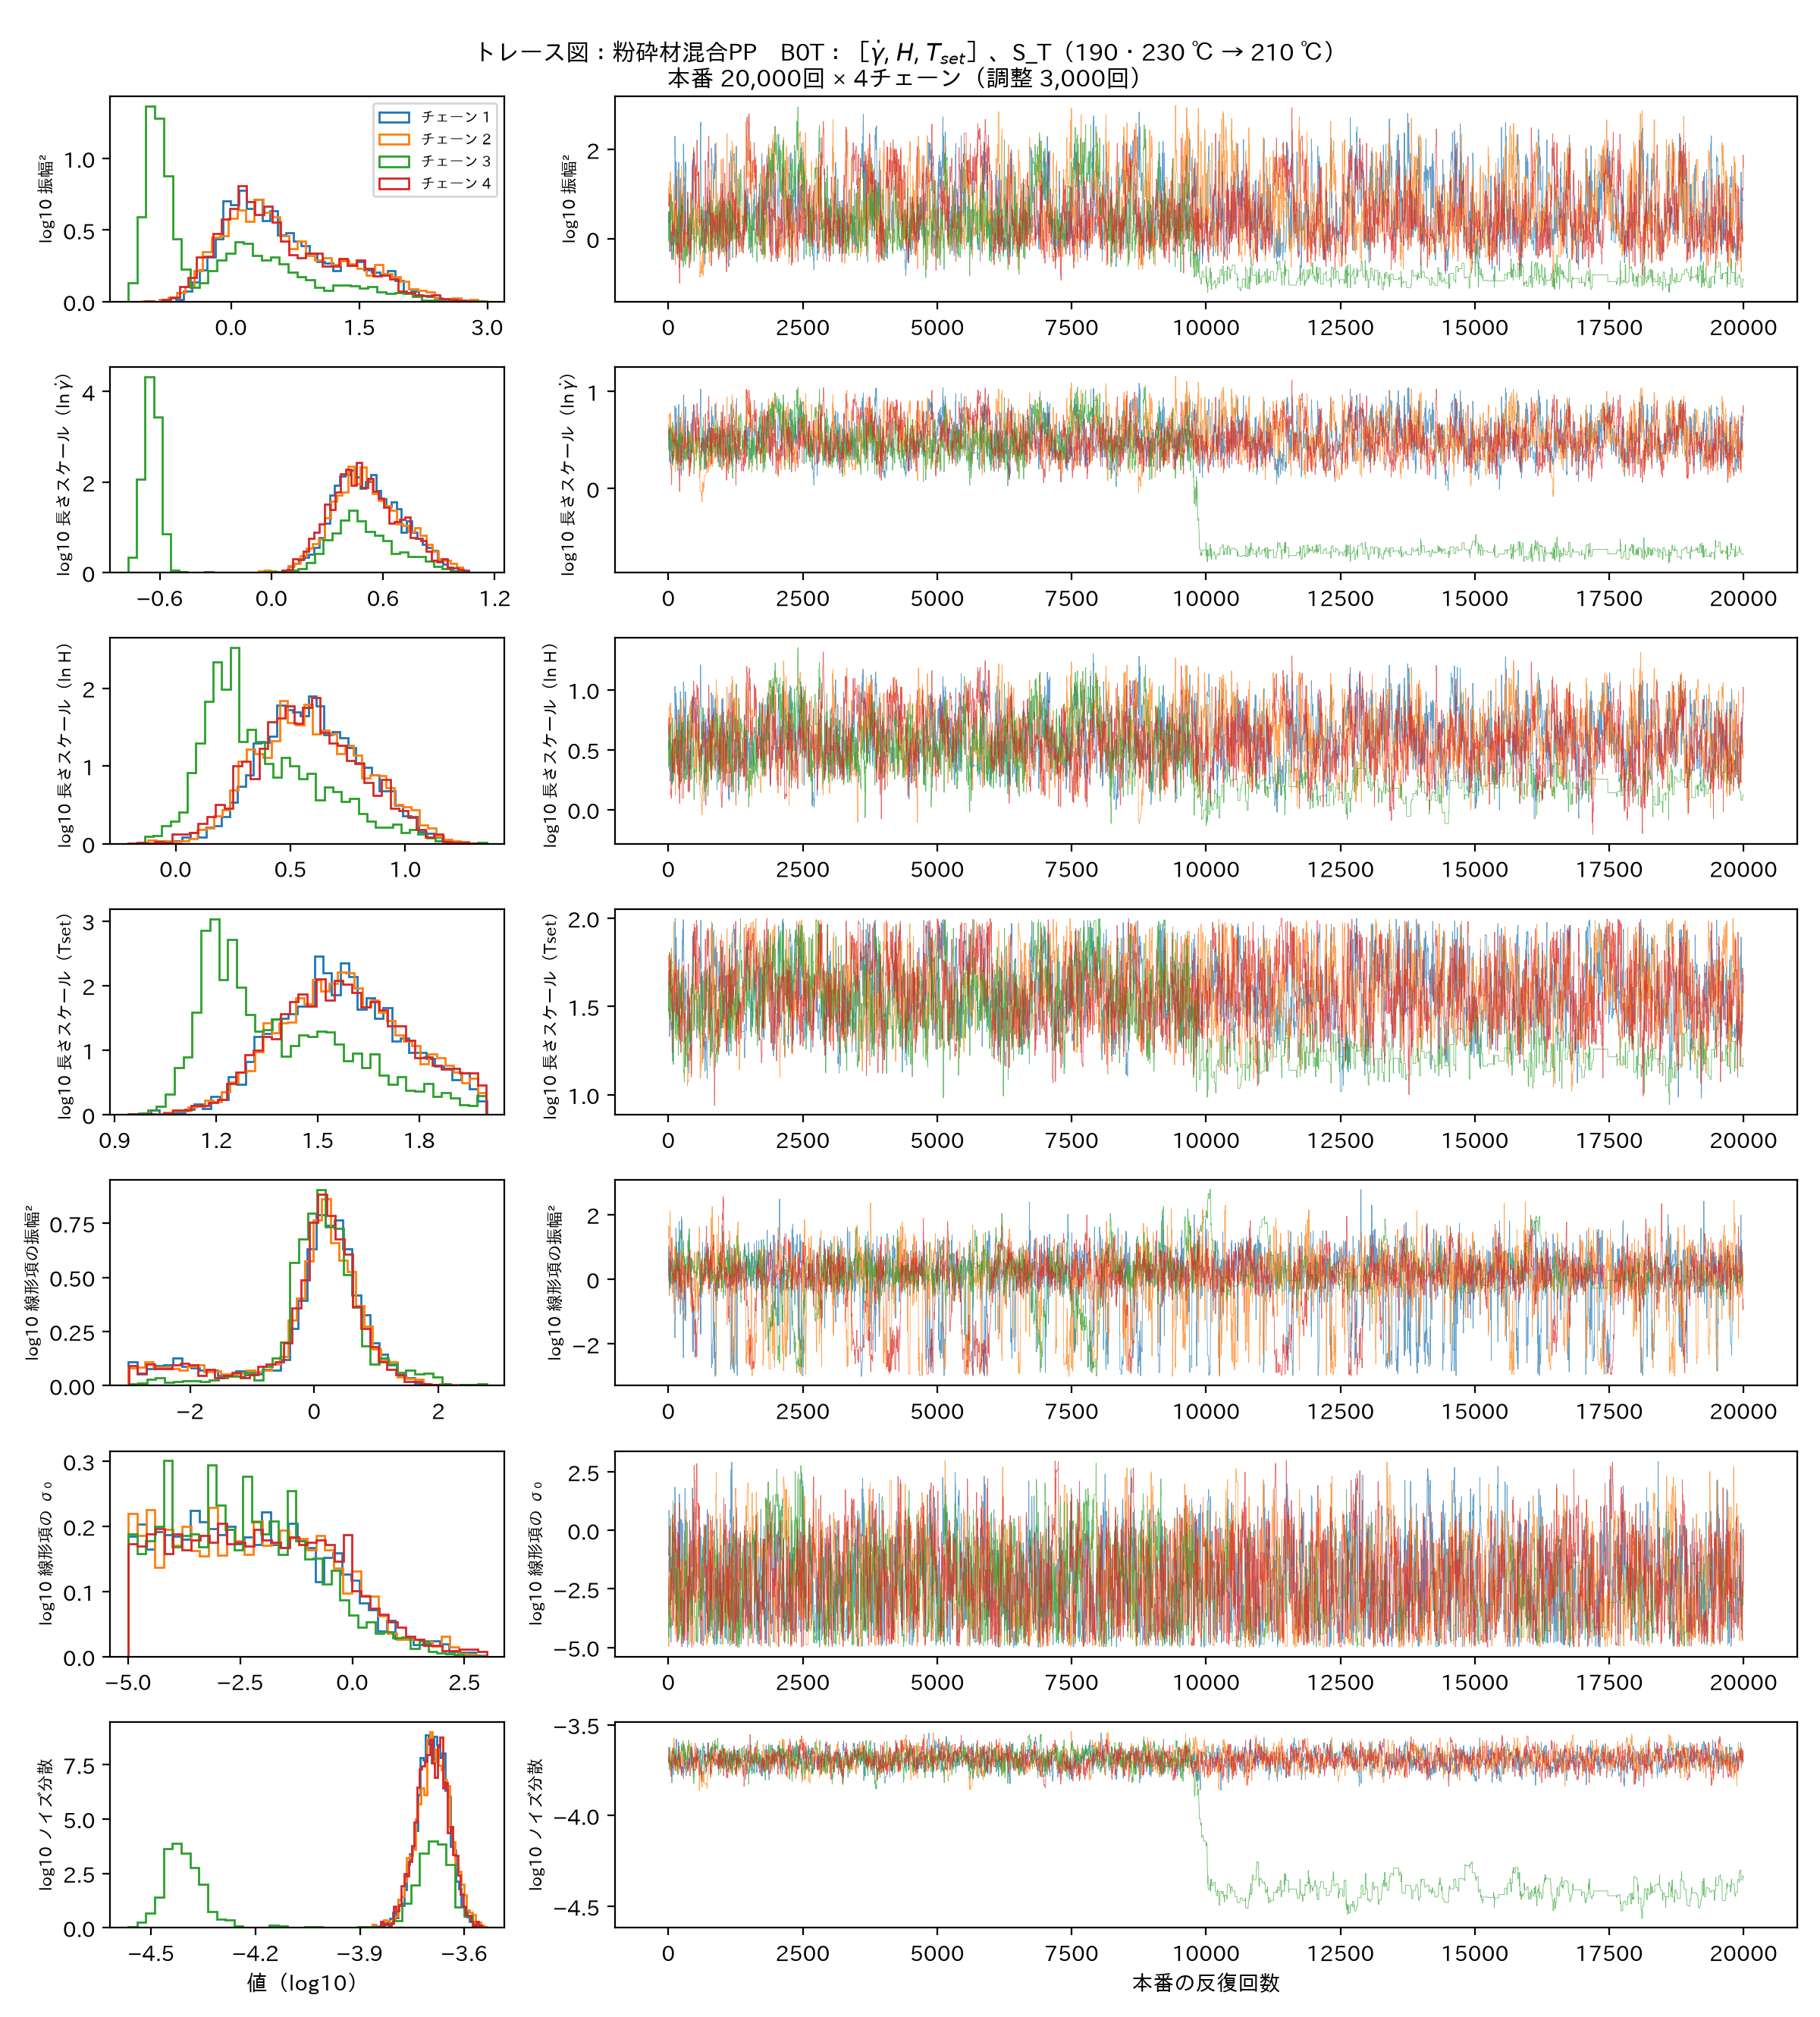
\includegraphics[width=0.78\linewidth]{fig_trace_S_T_MIX_B0T.png}
\caption{粉砕材混合 PP の B0T（S\_T の学習）のトレース図。チェーン 3 が、10,000 回ごろに別の山へ移っている}
\end{figure}
\begin{points}
\pt{ファイル}\file{results/step3c_mcmc/fig_trace_S_V_PP_B0T.png} のように、分割・材料・モデルごとに 1 枚（12 枚）。
\pt{何を示す図か}チェーンが、ちゃんと同じ分布を歩いているか（収束）を確かめる図です。ハイパーパラメータ 1 つにつき、1 行です。
\pt{軸と記号}左は、チェーンごとの分布（ヒストグラム）、右は、本番の反復ごとの値（足跡）。値は、$\log_{10}$（常用対数）。4 色がチェーン 1〜4。上から、振幅の 2 乗、各入力の長さスケール、線形項の振幅の 2 乗、線形項の $\sigma_0$、ノイズ分散。
\pt{見るポイント}右の足跡で、4 色が混ざり合って、同じ範囲を上下しているか。左の分布で、4 色が重なっているか。1 色だけ離れていれば、収束していません。
\pt{今回の結果}12 組のうち 11 組は、4 本のチェーンが混ざり合い、R-hat が 1.01 以下、ESS が 400 以上になりました（表\ref{tab:stats}）。最初の 8,000 回で ESS が足りなかった 4 組は、本番を 20,000 回に増やしました。収束の目安を満たさなかったのは、粉砕材混合 PP の B0T（S\_T の学習） の 1 組です。図のように、チェーン 3 が 10,000 回ごろに別の山（ノイズ分散が小さく、$\gd$ の長さスケールが短い解）へ移り、R-hat が 1.31、ESS が 10 になりました。B0T の事後分布には、「ショットごとの $\gd$ に細かく合わせる山」と「なめらかな山」があり、チェーンが行き来しにくいためです（多峰性）。この組の予測は、4 本をすべて混ぜて計算しているので、参考値として読みます。
\end{points}

% ---------------------------------------------------------------------
\subsection{事後分布と最尤推定値（\file{fig\_posterior\_vs\_mle\_*.png}）}
\begin{figure}[H]
\centering
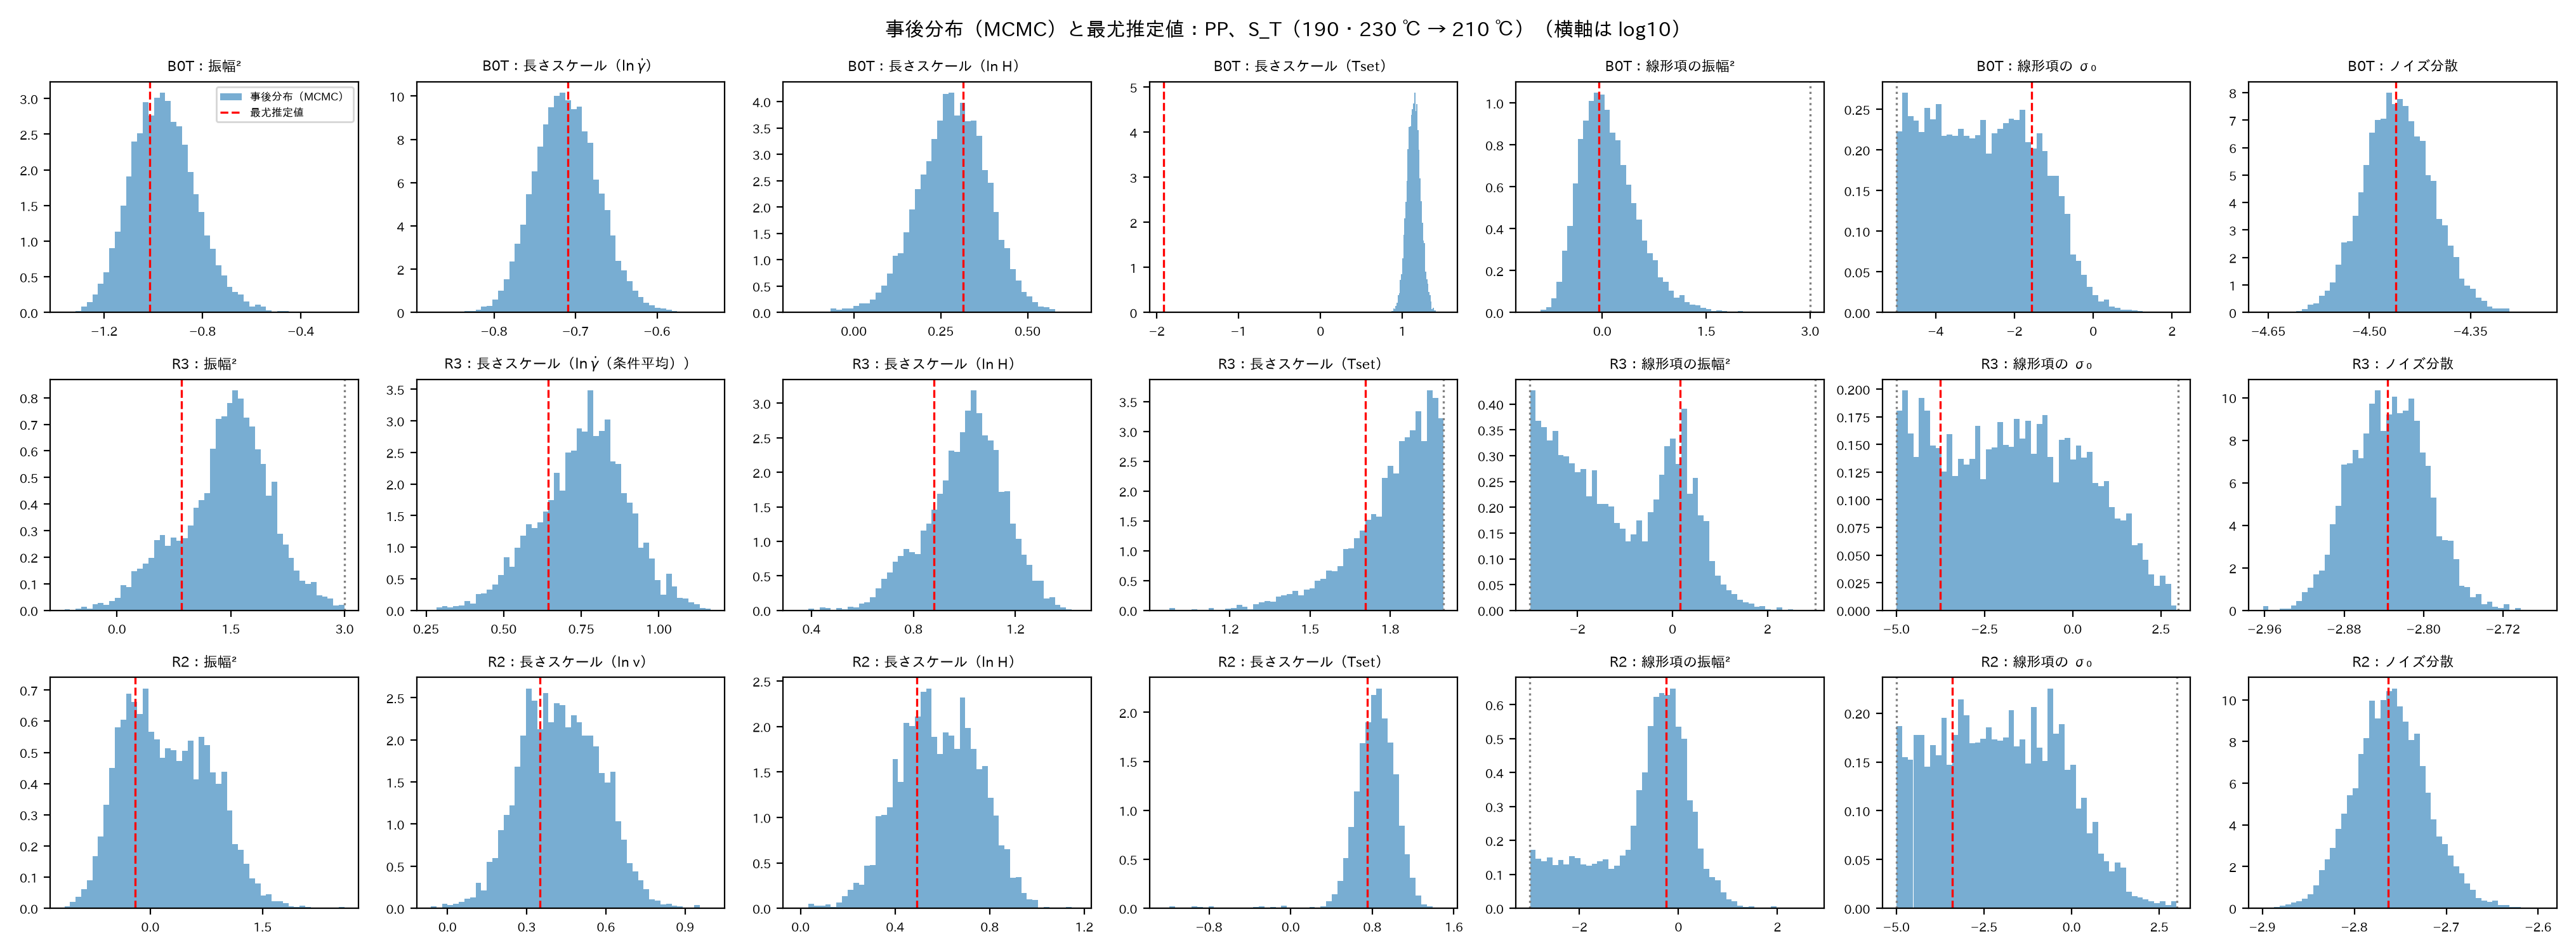
\includegraphics[width=\linewidth]{fig_posterior_vs_mle_S_T_PP.png}
\caption{PP（S\_T の学習）：事後分布（青）と最尤推定値（赤い破線）。灰色の点線は事前分布の範囲の端}
\end{figure}
\begin{points}
\pt{ファイル}\file{fig_posterior_vs_mle_S_V_PP.png}、\file{fig_posterior_vs_mle_S_T_PP.png}、\file{fig_posterior_vs_mle_S_V_MIX.png}、\file{fig_posterior_vs_mle_S_T_MIX.png}（材料と分け方ごとに 1 枚）。
\pt{何を示す図か}ハイパーパラメータの事後分布（山の形）と、最尤推定の値を比べる図です。行がモデル（B0T・R3・R2）、列がハイパーパラメータです。
\pt{軸と記号}横軸は値（$\log_{10}$）、青い棒が事後分布、赤い破線が最尤推定値、灰色の点線が、事前分布の範囲の端。
\pt{見るポイント}(1) 赤い破線が、青い山の中にあるか（最尤推定が、分布の中心付近か）。(2) 山が範囲の端（灰色の点線）に当たっていないか（端に当たれば、そのパラメータは、データだけでは決まらない）。
\pt{今回の結果}PP の B0T（S\_T の学習）では、$\Tset$ の長さスケールの最尤推定値が 0.012 で、事後分布の山（中央値 13.8、95\% 区間 9.5〜20.3）から大きく離れています（表\ref{tab:b0t}）。最尤推定は、確率のほとんどない谷に止まっていました。MCMC は、山の本体（長さスケール 約 14）を見つけます。R3 では、$\Tset$ の長さスケールの山が、上限（100）の近くにあります（中央値 約 70〜76）。$\Tset$ の効果が、Matern の部分ではなく、線形カーネルの部分で、ほぼ直線的に表されていることを意味します。事前分布の範囲の端に届いた R3 の 4 組は、この理由です。線形項の $\sigma_0$（右から 2 番目の列）は、範囲いっぱいに広がっていて、データでは決まりません（予測には、ほとんど効きません）。ほかのハイパーパラメータは、最尤推定の値が、山の中にあります。
\end{points}

% ---------------------------------------------------------------------
\subsection{図A：最尤推定と MCMC の比較}
\begin{figure}[H]
\centering
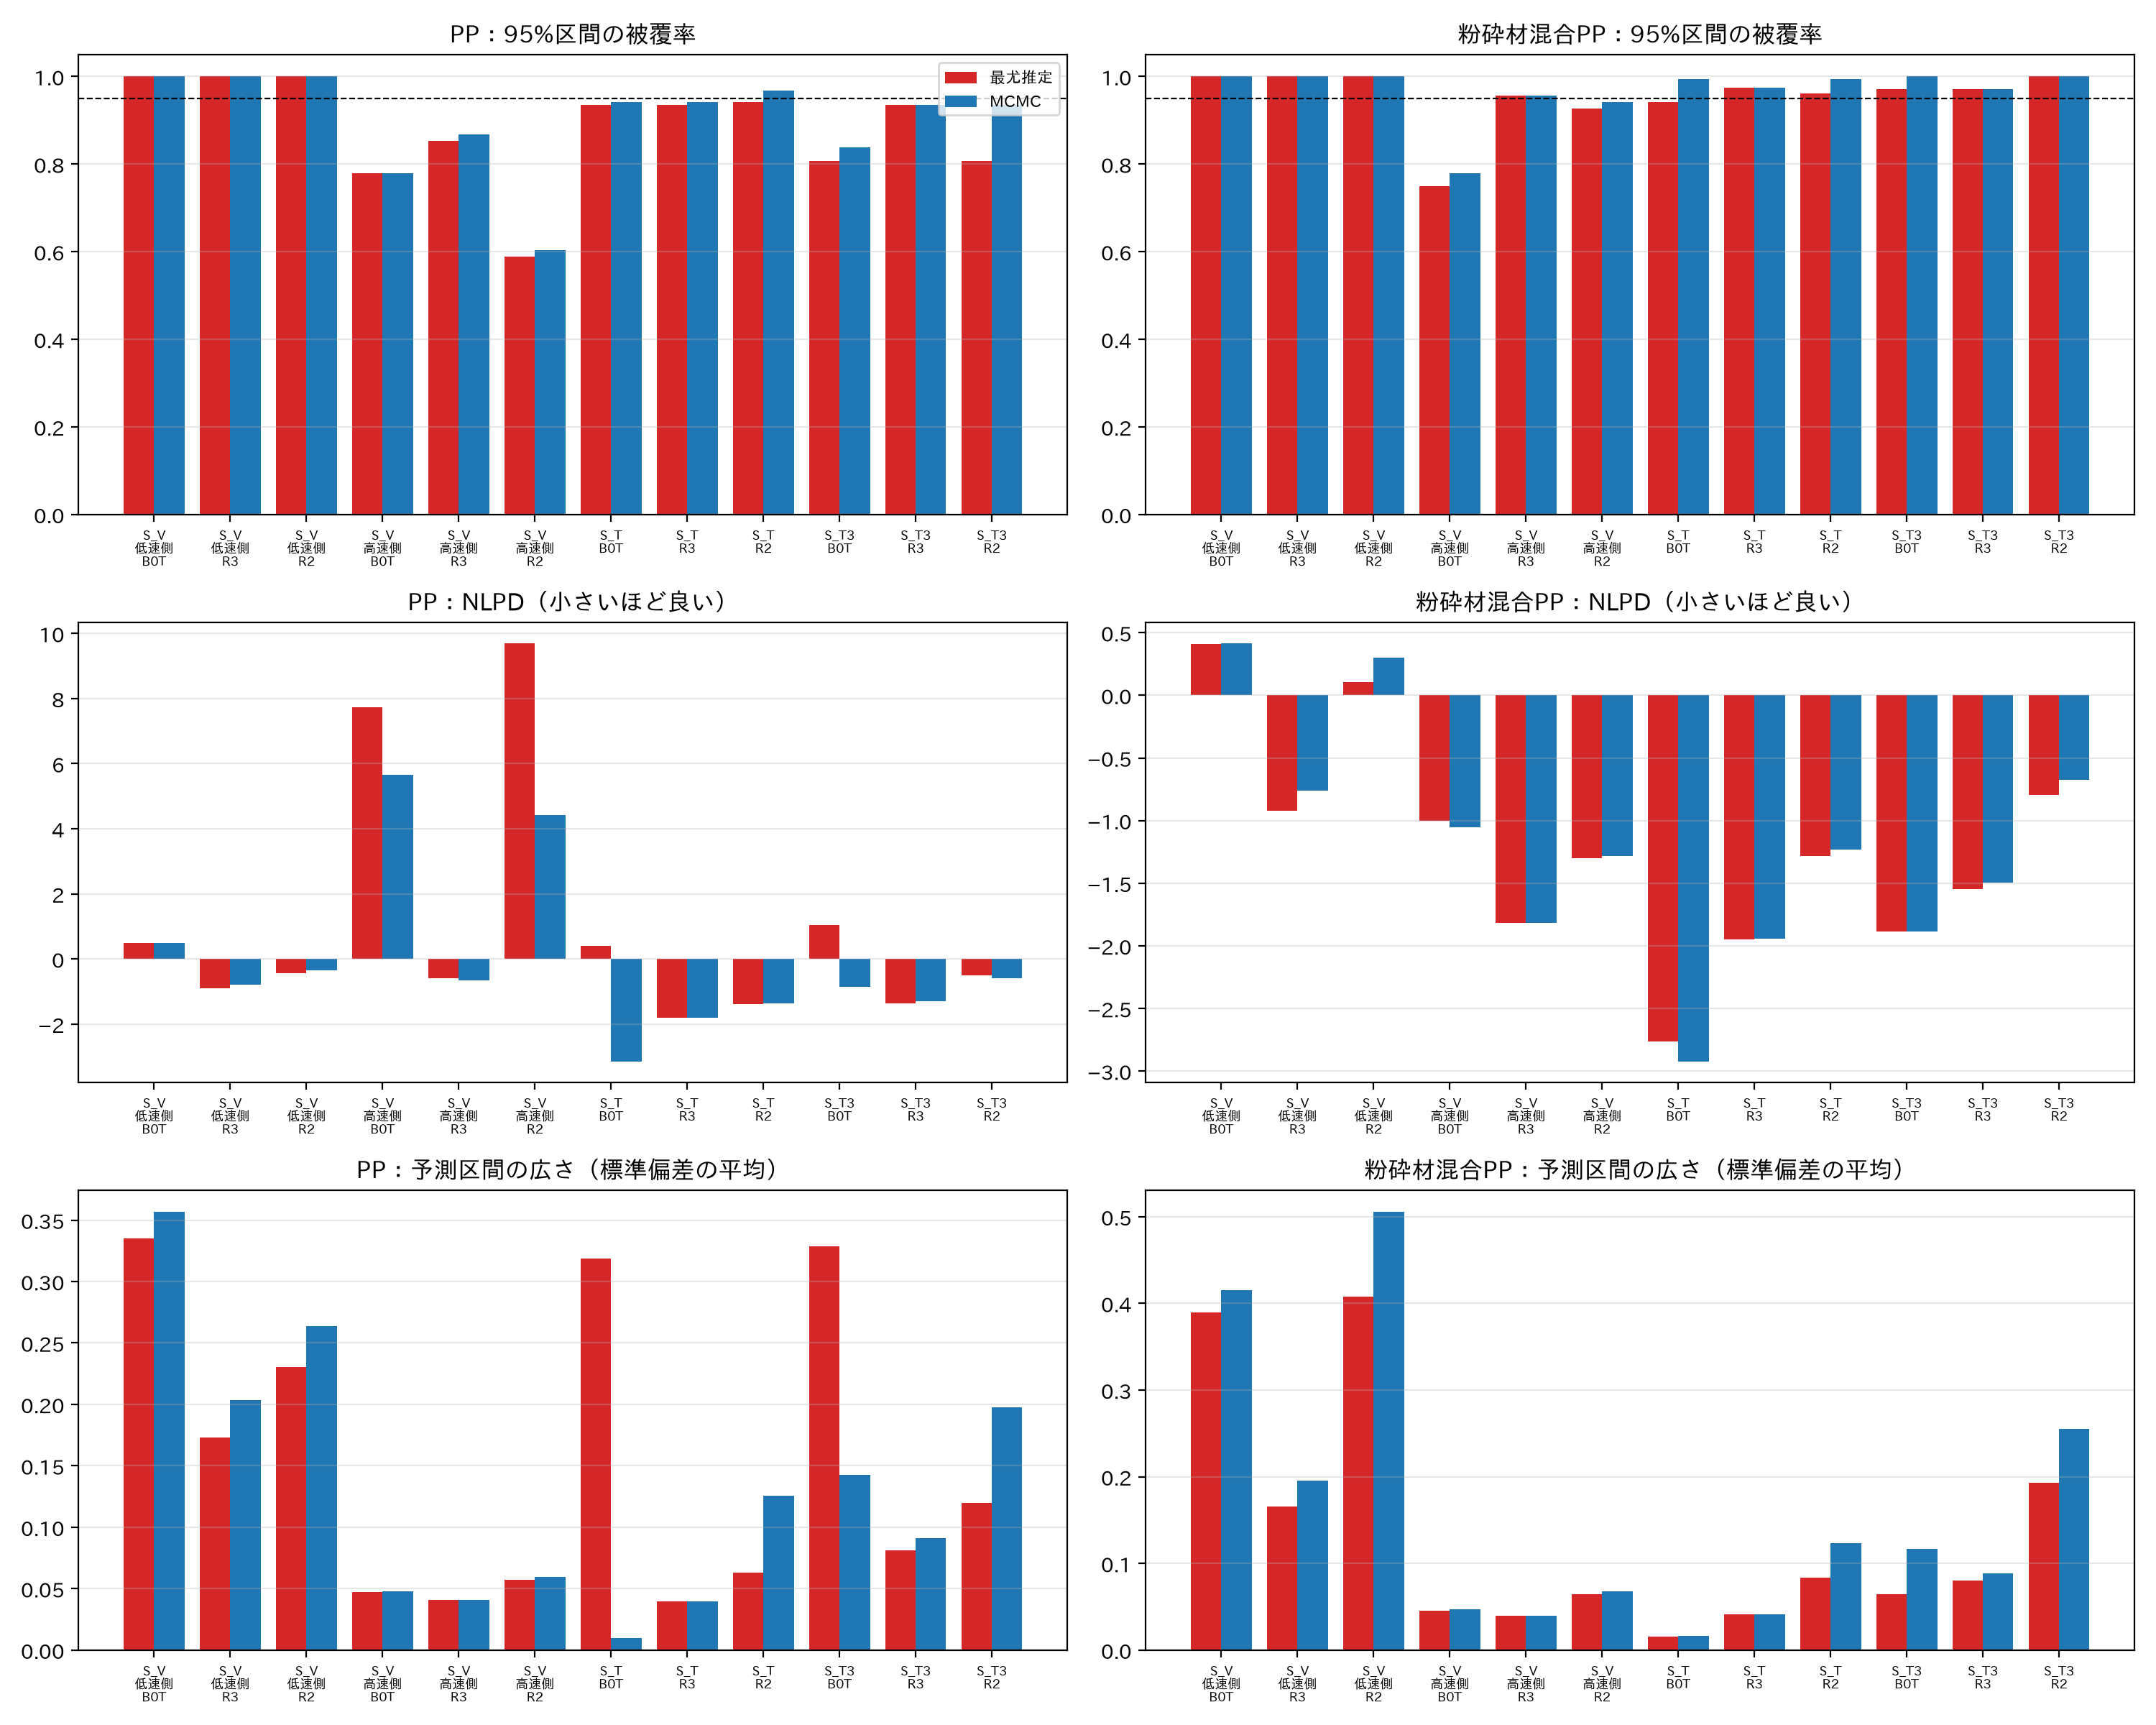
\includegraphics[width=0.95\linewidth]{figA_mle_vs_mcmc.png}
\caption{被覆率・NLPD・予測区間の広さの比較（赤：最尤推定、青：MCMC）}
\end{figure}
\begin{points}
\pt{ファイル}\file{results/step3c_mcmc/figA_mle_vs_mcmc.png}
\pt{何を示す図か}同じモデル・同じ検証データで、最尤推定と MCMC の予測を比べた図です。左が PP、右が粉砕材混合 PP。上段が 95\% 区間の被覆率、中段が NLPD、下段が予測区間の広さ（予測標準偏差の平均）。
\pt{軸と記号}横軸は、検証の種類（S\_V の低速側・高速側、S\_T、S\_T3）とモデル。赤い棒が最尤推定、青い棒が MCMC。被覆率の黒い破線は 0.95。
\pt{見るポイント}赤と青の棒が、ほぼ同じ高さなら、最尤推定で十分。青が低い NLPD なら、MCMC のほうが良い。区間の広さは、青が高ければ、ハイパーパラメータの不確かさが、予測の幅に入っています。
\pt{今回の結果}\textbf{R3}：高速側・S\_T は、最尤推定とほとんど同じです（NLPD の差 0.1 未満）。低速側（外挿）では、MCMC のほうが区間が約 1.2 倍広く（保守的）、NLPD が +0.11（PP）・+0.16（粉砕材混合 PP）と少し悪くなります。RMSE も、PP で 0.064 から 0.079、粉砕材混合 PP で 0.051 から 0.101 と、わずかに大きくなります。事後の平均は、直線的な傾きの不確かさ（線形項）を平均するため、低速側で、最尤推定よりやや外れやすくなるためです。最尤推定でも十分な精度です。\textbf{B0T}：PP の S\_T では、最尤推定が谷に止まっていたため、MCMC で RMSE が 0.362 から 0.010、NLPD が 0.41 から $-3.15$ へ、大きく改善します（区間の広さは 0.319 から 0.010）。\textbf{R2}：MCMC の区間は、S\_T で約 1.5〜2 倍と広くなり、PP の S\_V の高速側の NLPD は 9.70 から 4.42 へ改善します（P03 に引きずられる最尤推定より、広めの区間のため）。
\end{points}

% ---------------------------------------------------------------------
\subsection{図B：設定温度の効果の事後分布}
\begin{figure}[H]
\centering
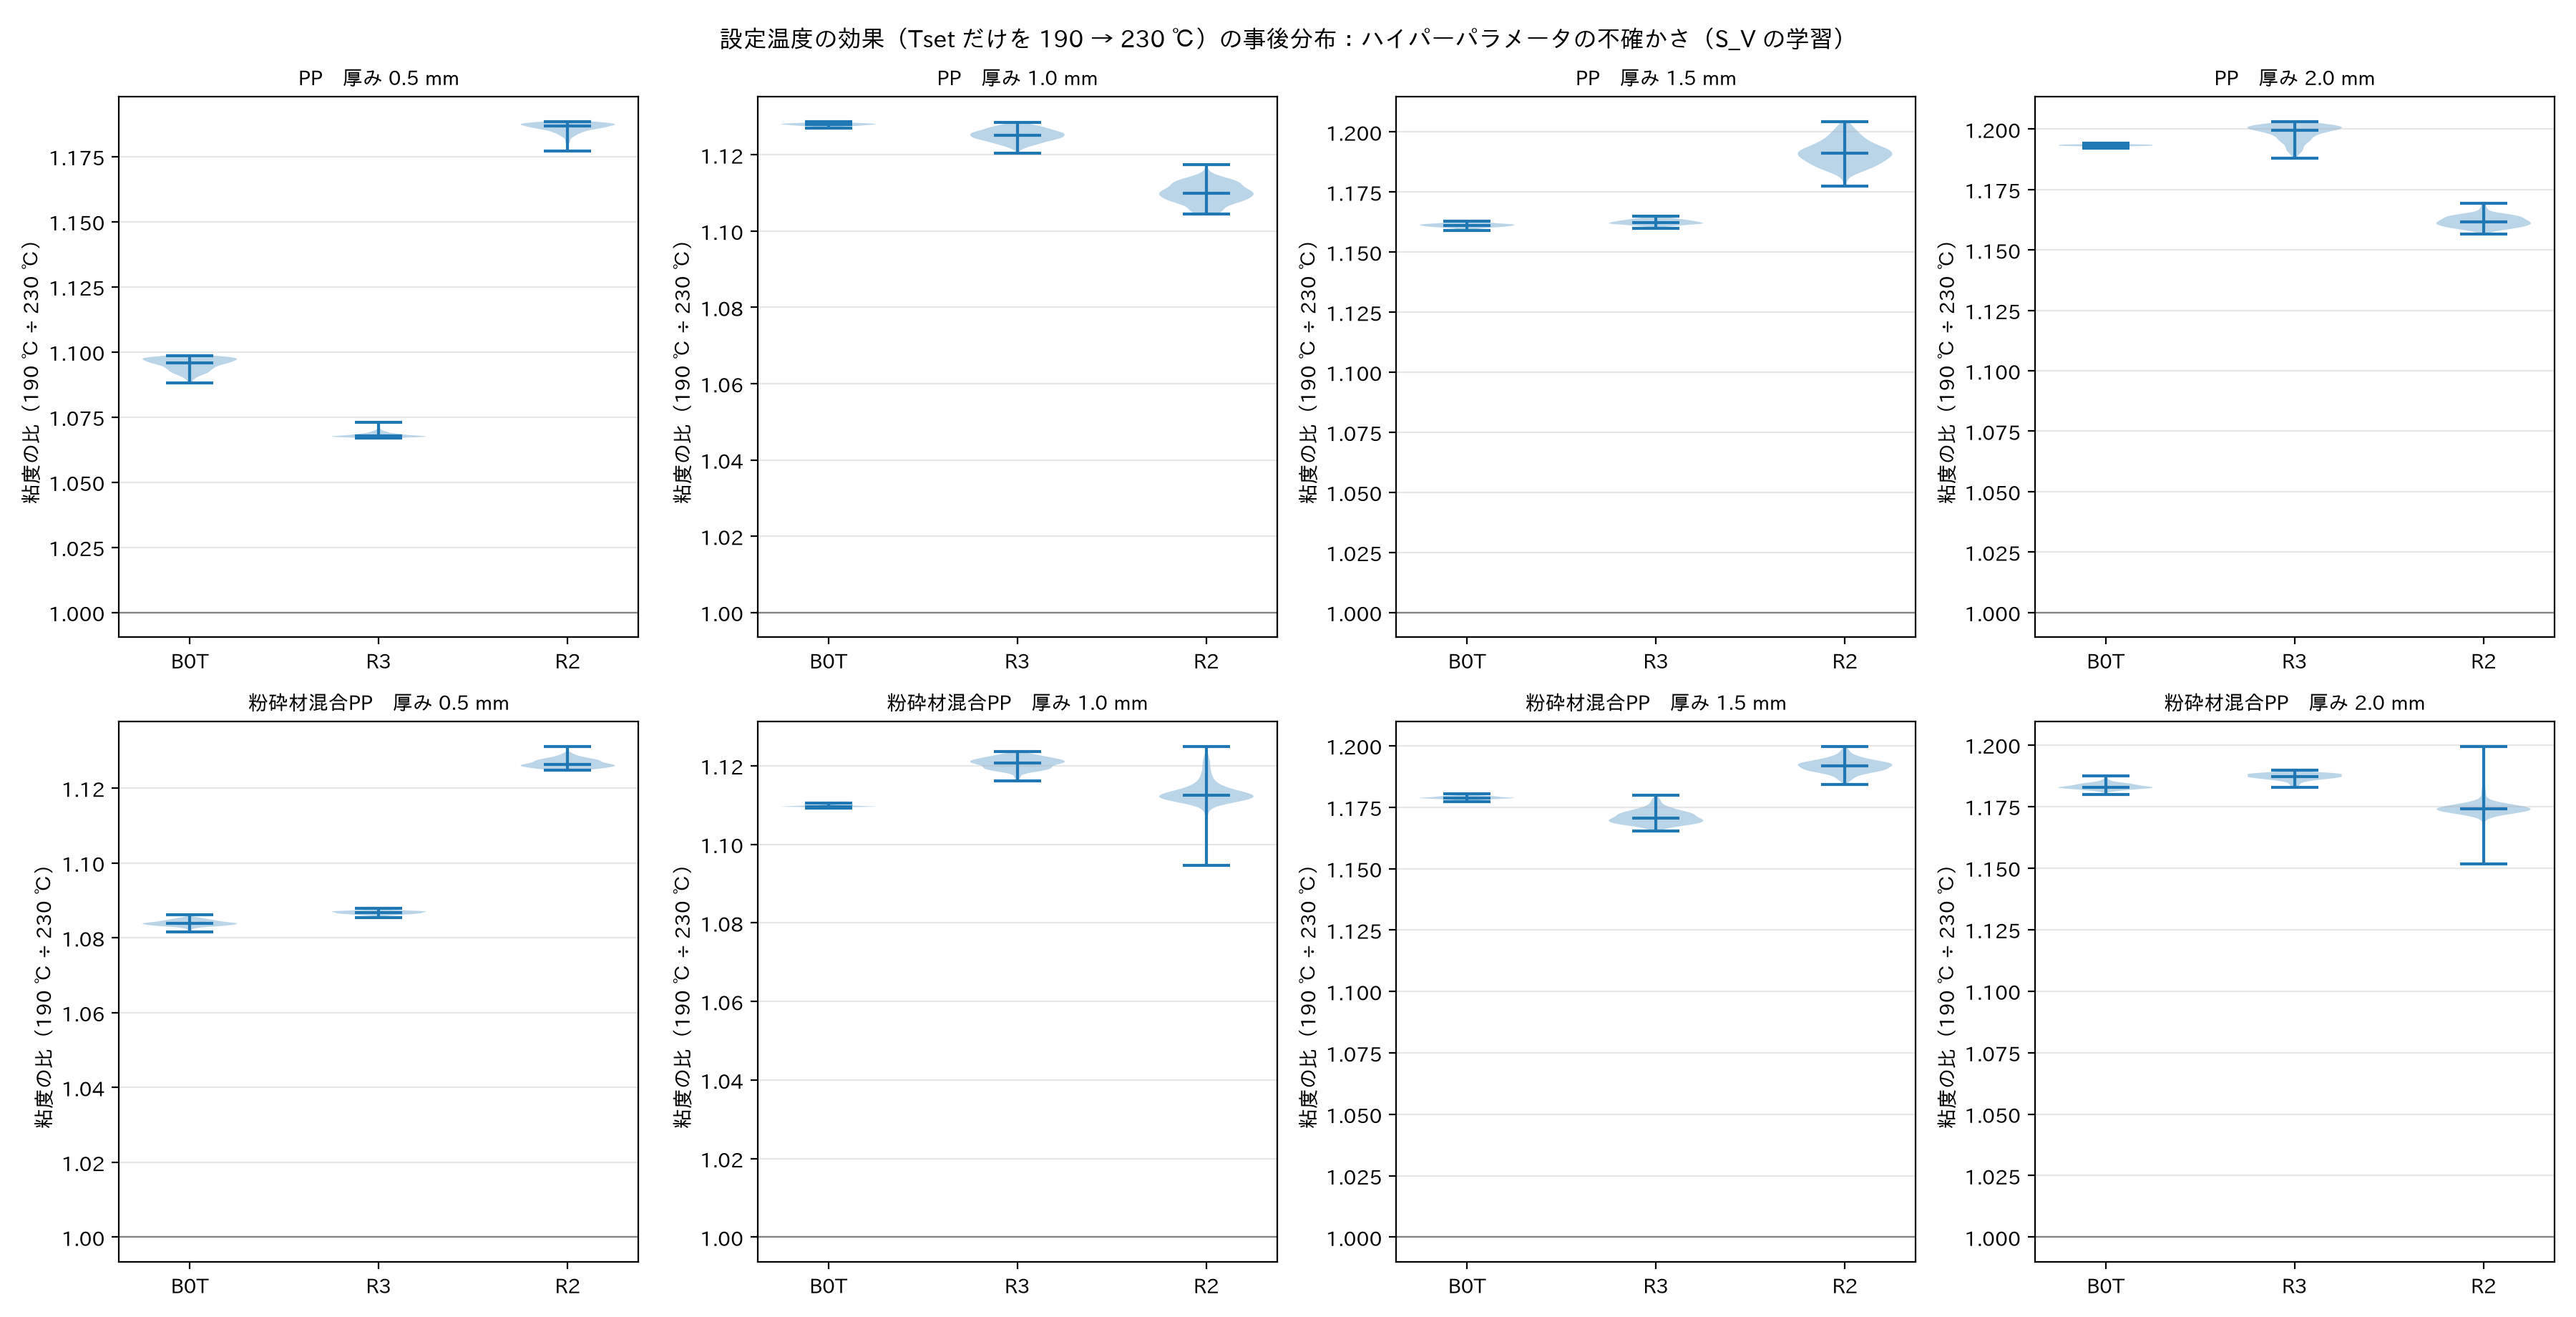
\includegraphics[width=0.95\linewidth]{figB_tset_effect_posterior.png}
\caption{Tset だけを 190 → 230 ℃ にした予測の粘度比の分布（ハイパーパラメータの不確かさによる）}
\end{figure}
\begin{points}
\pt{ファイル}\file{results/step3c_mcmc/figB_tset_effect_posterior.png}
\pt{何を示す図か}190 ℃ の粘度が 230 ℃ の何倍になるかの予測が、ハイパーパラメータの不確かさで、どれだけ変わるかを見る図です。
\pt{軸と記号}横軸がモデル、縦軸が粘度の比。バイオリンの形が、事後サンプルごとの比の分布。横線が、最小・中央値・最大。パネルは、厚みごと（上段 PP、下段 粉砕材混合 PP）。
\pt{見るポイント}形が細ければ、ハイパーパラメータが違っても、温度の効果は同じ。1 より上にあれば、190 ℃ のほうが粘い。
\pt{今回の結果}B0T と R3 の分布は、非常に細く、95\% 区間の幅が最大でも PP で 0.012、粉砕材混合 PP で 0.011 です。ハイパーパラメータの不確かさは、設定温度の効果（比 1.07〜1.20）にほとんど影響しません。R2 は、少し幅が広くなります（最大 0.019）。どのモデル・厚みでも、事後サンプルの 95\% 以上で、190 ℃ のほうが 230 ℃ より粘い（最小 1.00）という結果です。なお、この図は「ハイパーパラメータの不確かさ」だけを表します。予測そのものの不確かさ（予測区間）は、図Cで見ます。
\end{points}

% ---------------------------------------------------------------------
\subsection{図C：設定温度ごとの予測曲線（R3・B0T）}
\begin{figure}[H]
\centering
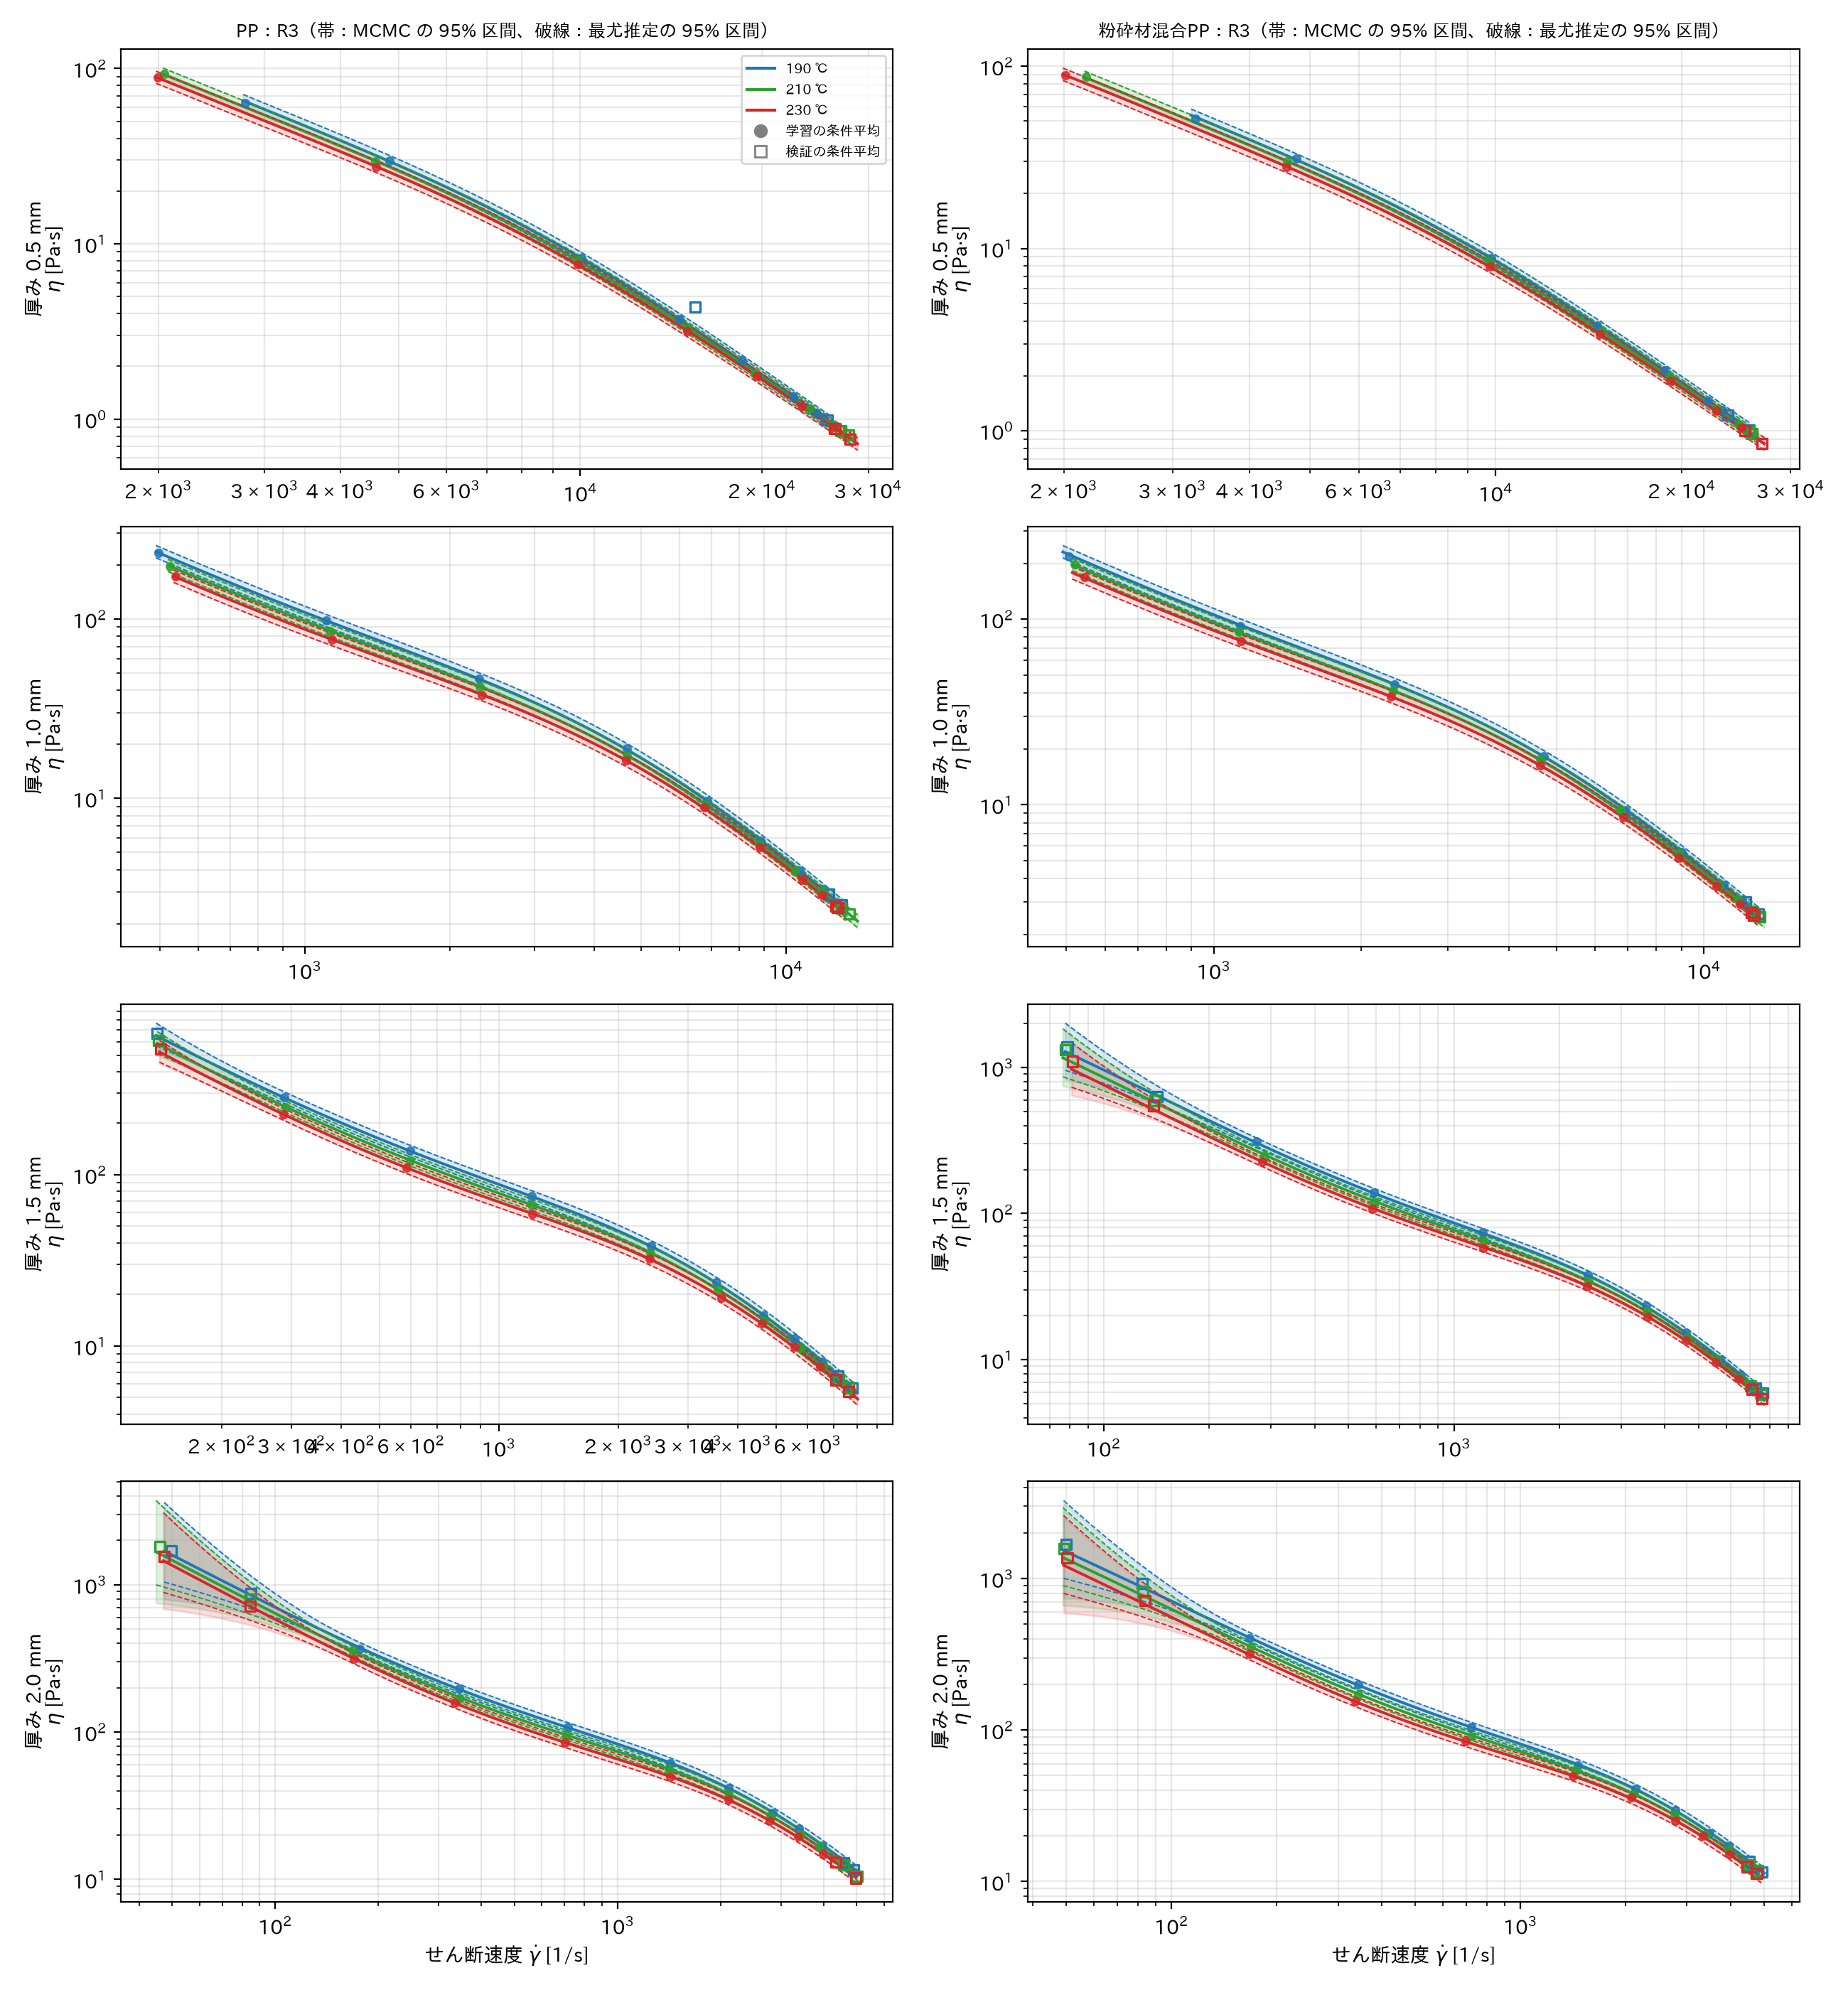
\includegraphics[width=0.72\linewidth]{figC_R3_curves.png}
\caption{R3：設定温度ごとの予測曲線。帯は MCMC の 95\% 区間、破線は最尤推定の 95\% 区間}
\end{figure}
\begin{points}
\pt{ファイル}\file{results/step3c_mcmc/figC_R3_curves.png}（R3）、\file{figC_B0T_curves.png}（B0T）
\pt{何を示す図か}5data で学習したモデルの、設定温度ごとの予測曲線を、MCMC の区間（帯）と最尤推定の区間（破線）で比べた図です。左が PP、右が粉砕材混合 PP、行が厚み。
\pt{軸と記号}横軸が $\gd$ [1/s]、縦軸が $\eta$ [Pa$\cdot$s]（対数軸）。色が設定温度（青 190 ℃、緑 210 ℃、赤 230 ℃）。丸が学習の条件平均、白抜きの四角が検証の条件平均。
\pt{見るポイント}帯と破線が、どれだけ違うか。検証の四角が、帯に入っているか。
\pt{今回の結果}R3 では、MCMC の帯（青・緑・赤）と最尤推定の破線が、ほとんど重なります。低速側（左端）では、帯が破線より少し広がります。検証の四角（外挿）は、帯の中に入ります。B0T は、曲線が波打ち、帯の幅も場所で変わります（ショットごとの $\gd$ を入力にしているため。手順3bの図1と同じ）。
\end{points}

% ---------------------------------------------------------------------
\subsection{高解像度のグラフ（報告書・発表資料用）}
\begin{points}
\pt{ファイル}\file{results/step3c_mcmc/highres/hr_<材料>_<モデル>_<学習>_mcmc_by-thickness_<厚み>mm.png}（厚みごと）と、\file{..._by-temperature_<温度>C.png}（設定温度ごと）。Git には入れません（ノートのセルで、いつでも作り直せます）。
\pt{何を示す図か}GPR6月のノートのセル9-2 と同じ見せ方の、せん断速度 ― 粘度の学習結果グラフを、\textbf{600 dpi（15 $\times$ 10 インチ）}で 1 枚ずつ保存します。MCMC の事後サンプル 200 個の予測を混ぜた分布で描き、線は予測の平均、帯は 95\% 予測区間、塗りつぶしの点は学習の条件、白抜きの点は検証の条件、黒い $\times$ は「感度確認」の条件です。既定は、R3（5data で学習）です。
\pt{変え方}ノート9章の「高解像度のグラフ」のセルの先頭に、設定エリアがあります（描くモデル・材料・学習の種類、レイアウト、帯、点、軸の範囲、図の大きさ・解像度、文字の大きさ、保存形式など）。\textbf{そのセルの設定だけを直して、そのセルだけを実行し直せます}（サンプリングはやり直しません。ノート全体を一度実行した後で）。
\end{points}

% =====================================================================
\section{表の見方}

\begin{table}[H]
\caption{サンプラーの統計（\file{sampler\_stats.csv}）。R-hat は最大、ESS は最小。採択率は 0.19〜0.28}\label{tab:stats}
\begin{tabularx}{\linewidth}{@{}l>{\raggedright\arraybackslash}p{3\zw}l>{\raggedright\arraybackslash}p{5\zw}rrrr@{}}
\toprule
材料 & 分割 & モデル & 本番の回数 & R-hat & ESS(bulk) & ESS(tail) & 端に届いた \\
\midrule
PP & S\_V & B0T & 8,000 & 1.007 & 911 & 917 & 0 \\
PP & S\_V & R3 & 20,000 & 1.008 & 1225 & 1492 & 1 \\
PP & S\_V & R2 & 20,000 & 1.004 & 1605 & 1063 & 0 \\
PP & S\_T & B0T & 20,000 & 1.005 & 1542 & 2876 & 0 \\
PP & S\_T & R3 & 8,000 & 1.008 & 440 & 411 & 1 \\
PP & S\_T & R2 & 8,000 & 1.006 & 480 & 535 & 0 \\
粉砕材混合 PP & S\_V & B0T & 8,000 & 1.009 & 936 & 1477 & 0 \\
粉砕材混合 PP & S\_V & R3 & 8,000 & 1.007 & 552 & 951 & 1 \\
粉砕材混合 PP & S\_V & R2 & 8,000 & 1.009 & 834 & 888 & 0 \\
粉砕材混合 PP & S\_T & B0T & 20,000 & 1.315 & 10 & 5 & 0 \\
粉砕材混合 PP & S\_T & R3 & 8,000 & 1.006 & 635 & 1040 & 1 \\
粉砕材混合 PP & S\_T & R2 & 8,000 & 1.008 & 799 & 1083 & 0 \\
\bottomrule
\end{tabularx}
\end{table}

\begin{table}[H]
\caption{最尤推定と MCMC の比較（検証データ。RMSE／NLPD／区間の広さ（予測標準偏差の平均）。\file{mle\_vs\_mcmc.csv}）}\label{tab:cmp}
\begin{tabularx}{\linewidth}{@{}l>{\raggedright\arraybackslash}p{5\zw}l*{6}{r}@{}}
\toprule
 & & & \multicolumn{2}{c}{RMSE} & \multicolumn{2}{c}{NLPD} & \multicolumn{2}{c}{区間の広さ} \\
\cmidrule(lr){4-5}\cmidrule(lr){6-7}\cmidrule(l){8-9}
材料 & 検証 & モデル & 最尤 & MCMC & 最尤 & MCMC & 最尤 & MCMC \\
\midrule
PP & S\_V 低速 & B0T & 0.474 & 0.469 & 0.50 & 0.48 & 0.335 & 0.357 \\
 &  & R3 & 0.064 & 0.079 & $-0.90$ & $-0.79$ & 0.173 & 0.203 \\
 &  & R2 & 0.161 & 0.197 & $-0.43$ & $-0.35$ & 0.231 & 0.264 \\
 & S\_V 高速 & B0T & 0.060 & 0.060 & 7.74 & 5.66 & 0.047 & 0.048 \\
 &  & R3 & 0.074 & 0.074 & $-0.59$ & $-0.66$ & 0.041 & 0.041 \\
 &  & R2 & 0.320 & 0.320 & 9.70 & 4.42 & 0.057 & 0.060 \\
 & S\_T & B0T & 0.362 & 0.010 & 0.41 & $-3.15$ & 0.319 & 0.010 \\
 &  & R3 & 0.039 & 0.039 & $-1.82$ & $-1.82$ & 0.039 & 0.040 \\
 &  & R2 & 0.060 & 0.061 & $-1.39$ & $-1.37$ & 0.063 & 0.125 \\
 & S\_T3 & B0T & 0.523 & 0.232 & 1.05 & $-0.86$ & 0.329 & 0.142 \\
 &  & R3 & 0.060 & 0.104 & $-1.38$ & $-1.31$ & 0.081 & 0.091 \\
 &  & R2 & 0.149 & 0.187 & $-0.50$ & $-0.60$ & 0.120 & 0.197 \\
粉砕材混合 PP & S\_V 低速 & B0T & 0.444 & 0.432 & 0.41 & 0.41 & 0.389 & 0.415 \\
 &  & R3 & 0.051 & 0.101 & $-0.92$ & $-0.76$ & 0.165 & 0.195 \\
 &  & R2 & 0.247 & 0.365 & 0.11 & 0.30 & 0.408 & 0.505 \\
 & S\_V 高速 & B0T & 0.056 & 0.056 & $-1.00$ & $-1.05$ & 0.045 & 0.047 \\
 &  & R3 & 0.039 & 0.039 & $-1.82$ & $-1.82$ & 0.039 & 0.040 \\
 &  & R2 & 0.066 & 0.068 & $-1.30$ & $-1.28$ & 0.064 & 0.068 \\
 & S\_T & B0T & 0.016 & 0.014 & $-2.76$ & $-2.92$ & 0.015 & 0.016 \\
 &  & R3 & 0.033 & 0.033 & $-1.95$ & $-1.94$ & 0.041 & 0.042 \\
 &  & R2 & 0.063 & 0.066 & $-1.28$ & $-1.23$ & 0.084 & 0.124 \\
 & S\_T3 & B0T & 0.178 & 0.208 & $-1.88$ & $-1.89$ & 0.064 & 0.116 \\
 &  & R3 & 0.043 & 0.069 & $-1.55$ & $-1.50$ & 0.080 & 0.088 \\
 &  & R2 & 0.166 & 0.231 & $-0.79$ & $-0.67$ & 0.193 & 0.255 \\
\bottomrule
\end{tabularx}
\end{table}

\begin{table}[H]
\caption{B0T の $\Tset$ の長さスケール（S\_T の学習。事後分布の要約。\file{posterior\_summary.csv}）}\label{tab:b0t}
\begin{tabularx}{\linewidth}{@{}l*{5}{r}@{}}
\toprule
材料 & 最尤推定 & 事後の中央値 & 2.5\% & 97.5\% & R-hat \\
\midrule
PP & 0.0121 & 13.8 & 9.48 & 20.3 & 1.001 \\
粉砕材混合 PP & 30.6 & 33.8 & 13.7 & 86.1 & 1.213 \\
\bottomrule
\end{tabularx}
\end{table}

\begin{table}[H]
\caption{\file{results/step3c\_mcmc/} の表}
\begin{tabularx}{\linewidth}{@{}>{\raggedright\arraybackslash}p{19\zw}X@{}}
\toprule
ファイル & 中身と主な列 \\
\midrule
\file{posterior_*.csv}（12 個） & 事後サンプル（対数）。\file{chain}、\file{draw}、各ハイパーパラメータ（\file{log_c}：振幅の 2 乗、\file{log_ls_*}：長さスケール、\file{log_c_lin}・\file{log_sigma0}：線形項、\file{log_noise}：ノイズ分散）、\file{lp}（対数事後密度）、\file{accepted}。 \\
\file{posterior_summary.csv} & ハイパーパラメータごとの事後分布の要約。\file{MLE}（最尤推定値）、\file{post_mean}、\file{median}、\file{q2.5}・\file{q97.5}、\file{r_hat}、\file{ess_bulk}、\file{ess_tail}、\file{post_at_bound}（範囲の端に届いたか）。 \\
\file{sampler_stats.csv} & 組み合わせごとのサンプラーの統計（採択率、最大 R-hat、最小 ESS、端に届いた数、時間）。 \\
\file{chain_info.csv} & チェーンごとの採択率・提案の大きさ・時間。 \\
\file{metrics.csv} & 最尤推定（MLE）と MCMC の指標（RMSE、R2、被覆率、NLPD、予測標準偏差）。\file{split}（S\_V・S\_T・S\_T3）、\file{subset}。 \\
\file{mle_vs_mcmc.csv} & 最尤推定と MCMC の差（NLPD の差、区間の広さの比）。 \\
\file{tset_effect_mcmc.csv} & 設定温度の効果（190/230 ℃ の粘度比）の、最尤推定・事後の中央値・2.5\%・97.5\%、1 を超える割合。 \\
\file{candidates.csv} & 候補のモデルと、選び方。 \\
\bottomrule
\end{tabularx}
\end{table}

% =====================================================================
\section{結果のまとめ}

\subsection{観点ごとの結論}
\begin{enumerate}[itemsep=0.6ex,topsep=0.6ex]
\item \textbf{収束}：12 組のうち 11 組が、R-hat 1.01 以下・ESS 400 以上を満たしました。満たさなかったのは、粉砕材混合 PP の B0T（S\_T の学習）です。多峰性（複数の山）のためで、予測には 4 本のチェーンの全サンプルを使いました。
\item \textbf{B0T は、MCMC で直る}：手順3bで、PP の S\_T の B0T は、最尤推定が谷に止まり、210 ℃ を外しました（RMSE 0.362）。MCMC は、山の本体を見つけ、RMSE 0.010、NLPD $-3.15$ になりました（図A、表\ref{tab:cmp}）。ただし、B0T の事後分布は多峰性で、扱いにくいモデルです。
\item \textbf{R3 は、最尤推定で十分}：R3 の MCMC と最尤推定は、高速側・S\_T でほぼ同じ（NLPD の差 0.1 未満）です。低速側では、MCMC の区間が約 1.2 倍広く（外挿で、広めになるのは妥当）、NLPD は +0.11（PP）・+0.16（粉砕材混合 PP）と、少し悪くなります。ハイパーパラメータが 1 つの山に決まる R3 では、1 組で近似して問題ありません。
\item \textbf{R2（設定値だけ）は、MCMC で区間が広がる}：S\_T で約 1.5〜2 倍。実測の $\gd$ を使わない分、不確かさが大きいことを、区間が表しています。
\item \textbf{決まらないパラメータ}：線形項の $\sigma_0$ は、データで決まらず、事前の範囲いっぱいに広がります（予測にはほとんど効きません）。R3 の $\Tset$ の長さスケールは、上限（100）に近く、温度の効果が、ほぼ直線的（線形項）で表されています。
\item \textbf{設定温度の効果は、ハイパーパラメータによらない}：190/230 ℃ の粘度比の 95\% 区間の幅は、B0T・R3 で 0.02 未満です（図B）。
\item \textbf{結論}：基本モデル（R3）は、最尤推定でよく、MCMC は、最適化が不安定なモデル（B0T）の確認と、区間を広めに見たいときに使います。手順5の本実装で、MCMC を使うかは、構造（5a）が決まってから相談します。
\end{enumerate}

\subsection{次の手順}
\begin{points}
\pt{手順5a}温度のシフト構造の見直しです（別の説明書）。ここで確かめた、「条件平均の $\gd$ を入力にした R3 は、最尤推定でも十分」という結論は、5a の評価（ショット単位の GPR の最尤推定）にも使えます。
\pt{手順5（本実装）}5a の結果を見て決めます。最終モデルでは、MCMC を使うかを、そこでまた相談します。
\end{points}

\end{document}
